% Results section. Source: manuscript.md (Results).
% Every number is copied verbatim from the manuscript; do not edit digits here.
\section{Results}\label{sec:results}

Each result is a controlled validation in a known model; we report the grounded
number and its producing script.

\subsection{R0 --- order alone}\label{sec:r0}

\textbf{Dimension.} In the declared flat Poisson-sprinkling model, the
Myrheim--Meyer order statistic estimates spacetime dimension, as in earlier
tests on flat and conformally flat spacetimes~\cite{reid2003}: for true
dimension 2 the estimate moves $1.95 \to 2.03 \to 2.01 \to 1.99$ at
$N = 300$, 600, 1200, 2400; for dimension 3, $2.96 \to 2.95 \to 3.00 \to 3.00$;
for dimension 4, $4.07 \to 3.97 \to 3.93 \to 3.97$. Endpoint RMSE is lower at
$N = 2400$ than at $N = 300$, with non-monotonic finite-sample fluctuations for
dimensions 3 and 4 (\expid{exp10};
\artifact{outputs/\allowbreak{}data/\allowbreak{}dimension\_\allowbreak{}reconstruction\_\allowbreak{}summary.csv}).

\textbf{Uncalibrated timelike statistic (longest chain).} The longest chain
follows the Brightwell--Gregory scaling $L \sim \sqrt{2\rho}\,\tau$, approached
from below at finite density: at $\rho = 300$ the normalized length
$L/(\sqrt{\rho}\,\tau)$ is 1.325 with endpoints included and 1.085 with
endpoints removed, versus the asymptotic $\sqrt{2} \approx 1.414$. The
proper-time estimator reads the endpoint-exclusive length, and its mean error
there is $-0.127$; the same chains scored under the inclusive convention give
$-0.046$, the two separated by the exact offset $2/\sqrt{2\rho} = 0.082$. At
this density the median chain carries 12.5 elements including its endpoints,
so the two-element difference between the two conventions accounts for most of
that residual: at these chain lengths it is a convention effect before it is a
finite-size one (\expid{exp09};
\artifact{outputs/\allowbreak{}data/\allowbreak{}longest\_\allowbreak{}chain\_\allowbreak{}calibration\_\allowbreak{}summary.csv}). The approach
toward the asymptotic value with $N$ is shown by the chain estimator's error
falling with $N$ in \sref{sec:r1}. Raw longest-chain length is order-theoretic.
Interpreting it as proper time, including the normalization quoted here,
belongs to R1 because it requires density and a dimension-specific asymptotic
law; absolute scale is not fixed by order alone.

\subsection{R1 --- order plus measure: timelike proper time}\label{sec:r1}

With event density supplied, Alexandrov interval cardinality reconstructs
timelike proper time between internal pairs,
$\tau_{\mathrm{est}} = \sqrt{2K/\rho}$. The volume-estimator relative RMSE
falls from 0.273 at $N = 300$ to 0.105 at $N = 2400$. Its separately
aggregated RMSE is below the chain estimator's ($0.382 \to 0.231$) at every
$N$, but the volume statistic uses 500 pairs per $N$ whereas the chain
statistic uses 125, so this is not a paired comparison, and the chain
estimator additionally carries the endpoint-convention offset of
\sref{sec:r0}, so the comparison is not convention-free either
(\expid{exp07};
\artifact{outputs/\allowbreak{}data/\allowbreak{}timelike\_\allowbreak{}pair\_\allowbreak{}reconstruction\_\allowbreak{}summary.csv}). In a
fixed-interval sanity check, the interval-cardinality formula returns
$\tau = 2.0$ exactly because the full sampling diamond uses $K = N$ and
$\rho = N/V$; this is a normalization identity, not an independent accuracy
test. The chain estimate converges toward it (0.303 at $N = 200$ to 0.0125 at
$N = 2000$) (\expid{exp03};
\artifact{outputs/\allowbreak{}data/\allowbreak{}timelike\_\allowbreak{}reconstruction\_\allowbreak{}summary.csv}). The observed
errors are consistent with finite-sampling noise at the tested settings: the
ratio of reconstruction RMSE to the predicted Poisson standard deviation is
0.93--1.07 across $N$ (binomial 1.00--1.14). Smaller bias or other estimator
errors are not excluded (\expid{exp08};
\artifact{outputs/\allowbreak{}data/\allowbreak{}probe\_\allowbreak{}pair\_\allowbreak{}statistical\_\allowbreak{}calibration\_\allowbreak{}summary.csv}).

\subsection{R2 --- order plus observer: radar time and unsigned distance}\label{sec:r2}

Given an observer chain with clock labels, radar time and unsigned radar
distance are reconstructed from causal accessibility; at $N = 300$ the error
falls roughly by half per doubling of tick resolution---radar-time RMSE from
0.027 at 16 ticks to 0.0033 at 128 ticks, radar-distance RMSE from 0.071 to
0.0085, with the accessible fraction 1.0 throughout (\expid{exp11};
\artifact{outputs/\allowbreak{}data/\allowbreak{}discrete\_\allowbreak{}radar\_\allowbreak{}reconstruction\_\allowbreak{}summary.csv}). A single
observer determines only unsigned distance (the reflection degeneracy of
\sref{sec:negative}).

\subsection{R3 --- plus orientation: signed coordinates and the Lorentz map}\label{sec:r3}

A second synchronized beacon chain with known separation supplies orientation,
lifting the degeneracy to signed $(1{+}1)$D coordinates. The affine map
recovered between two oriented inertial protocols approaches the Lorentz
boost, with the fitted-$\beta$ RMSE falling with tick density. Averaged over
$N$ as in \fref{fig:convergence}, it falls from 0.00495 at 32 ticks to
0.000975 at 128 ticks for $\beta = 0.3$, and from 0.01345 to 0.00431 for
$\beta = 0.6$ (\expid{exp13};
\artifact{outputs/\allowbreak{}data/\allowbreak{}oriented\_\allowbreak{}radar\_\allowbreak{}lorentz\_\allowbreak{}summary.csv}).

\Fref{fig:convergence} collects the convergence behaviour of the first four
rungs: dimension recovery (a), timelike proper time (b), observer radar (c),
and Lorentz-map recovery (d).

\begin{figure}[t]
\centering
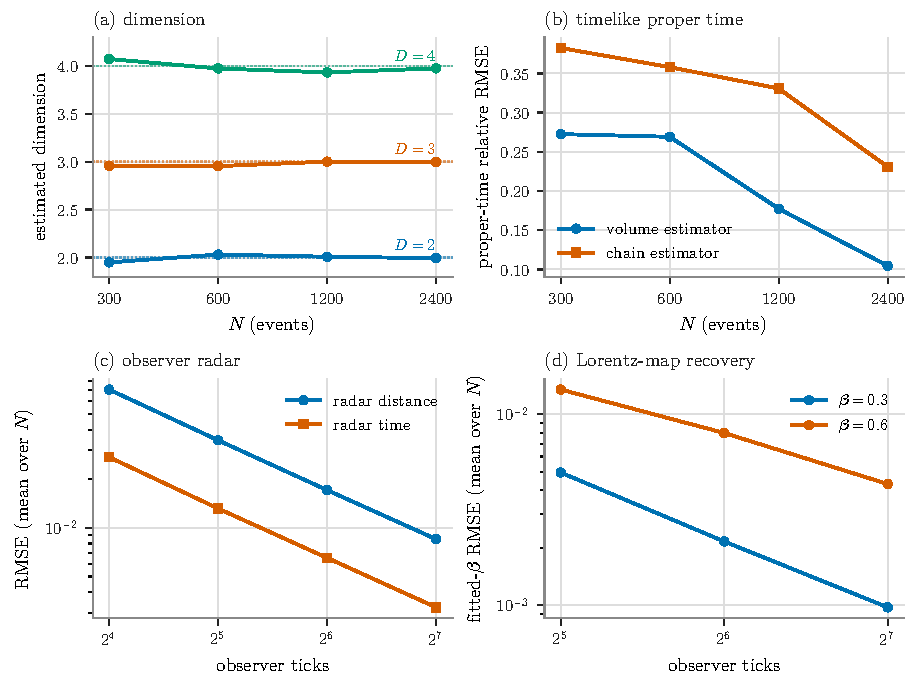
\includegraphics[width=0.95\textwidth]{figures/fig2_convergence.pdf}
\caption{Reconstruction accuracy in controlled models. (a) Myrheim--Meyer
dimension estimates lie near $D = 2$, 3, 4; endpoint RMSE is lower at
$N = 2400$ than $N = 300$ despite non-monotonic finite-sample fluctuations
(\expid{exp10}). (b) Timelike proper-time relative RMSE falls with $N$, the
interval-volume estimator below the separately aggregated longest-chain
estimator (\expid{exp07}). (c) Observer radar time and distance RMSE fall
about by half per doubling of clock ticks (\expid{exp11}). (d) Recovered
Lorentz $\beta$ RMSE falls with clock ticks for two boosts (\expid{exp13}).
Panels (c, d) are means over $N$; axes are logarithmic where noted.}
\label{fig:convergence}
\end{figure}

\subsection{R4 --- plus oriented atlas: transition-map consistency}\label{sec:r4}

With overlapping observer charts that retain the synchronized, calibrated
orientation reference from R3, affine Lorentz/Poincar\'e transition maps fit
on chart overlaps show approximately consistent composition and invariant
agreement, improving with tick density: the mean transition-map $\beta$ error
falls $0.0047 \to 0.0012$ and the invariant-interval RMSE $0.050 \to 0.010$
(ticks $32 \to 128$), while loop closure ($A \to B \to C$ versus direct
$A \to C$) has a $\beta$-composition error of $0.0072 \to 0.0017$
(\expid{exp14};
\artifact{outputs/\allowbreak{}data/\allowbreak{}observer\_\allowbreak{}atlas\_\allowbreak{}transition\_\allowbreak{}summary.csv},
\artifact{outputs/\allowbreak{}data/\allowbreak{}observer\_\allowbreak{}atlas\_\allowbreak{}loop\_\allowbreak{}summary.csv}). On exact analytic
input the same transition/loop machinery recovers the maps to machine
precision ($\beta$ error ${\sim}5.6\times10^{-17}$, RMSE
${\sim}4\times10^{-17}$) (\expid{exp15};
\artifact{outputs/\allowbreak{}data/\allowbreak{}exact\_\allowbreak{}poincare\_\allowbreak{}map\_\allowbreak{}sanity.csv}).

\subsection{R5 --- plus conformal measure: volume and coarse-graining}\label{sec:r5}

Positive conformal rescalings preserve causal order while changing volume and
clock scale: under constant (1.0/1.5/2.0) and sinusoidal rescalings the causal
matrix is unchanged and the reconstructed dimension is identical (2.020),
while the proper-time ratio tracks 1.0/1.5/2.0 and the volume ratio
1.0/2.25/4.0 (\expid{exp18};
\artifact{outputs/\allowbreak{}data/\allowbreak{}conformal\_\allowbreak{}order\_\allowbreak{}ambiguity\_\allowbreak{}summary.csv}). Two
different things must therefore be supplied, and they fail differently when
withheld: a scale (M, one number) and a shape (W, a field). The profile
\expid{exp19} tests is genuinely position-dependent---$\Omega(t) = 1 +
0.3\sin(\pi t/T)$ moves the local volume element by a factor of 3.45 across
the diamond (0.49 to 1.69) while leaving every global summary near flat: the
diamond volume moves by 2.7\% (\expid{exp18}'s sinusoidal row). A
reconstruction holding only the global density therefore has almost no bias
to correct (unweighted volume bias $-0.0057$ to $-0.0028$), but it carries a
position-dependent error that no single rescaling removes: its relative RMSE
stalls at $0.373 \to 0.298 \to 0.300$ across the tested $N$. Supplying the
local weights removes the floor: the weighted relative RMSE falls
$0.235 \to 0.176 \to 0.119$, tracking the flat-profile sampling floor
($0.234 \to 0.174 \to 0.118$) to within 1.3\%, and the
unweighted-to-weighted volume-RMSE ratio grows $2.0 \to 2.8 \to 4.3$ with
$N$---the signature of a removed systematic rather than of reduced noise.
What R5 demonstrates is the replacement of a non-vanishing error floor by
flat-case, noise-limited error scaling---a consistency statement, not a bias
correction (\expid{exp19};
\artifact{outputs/\allowbreak{}data/\allowbreak{}weighted\_\allowbreak{}conformal\_\allowbreak{}volume\_\allowbreak{}summary.csv}).

The constant-1.5 profile in the same table is a control, not the result: a
constant weight rescales estimate and truth alike, so its weighted relative
RMSE equals the flat profile's at every tested $N$, and its unweighted bias
(${\sim}{-0.29}$) is exactly the missing global factor---a normalization
identity in the sense of \sref{sec:r1}, whose repair is R1's ingredient M,
not W. The analytic volume/proper-time formulas are verified to
${\sim}1\times10^{-7}$ (\expid{exp20};
\artifact{outputs/\allowbreak{}data/\allowbreak{}conformal\_\allowbreak{}volume\_\allowbreak{}exact\_\allowbreak{}sanity.csv}). Under random
thinning, density-rescaled reconstruction is stable (volume RMSE
$0.018 \to 0.009$, dimension steady ${\sim}2.0$) while the uncorrected
estimate blows up to RMSE 0.270 (bias $-0.183$) at 25\% retention. The
thinning is uniform, so its keep probability is a single global scalar: a
robustness statement about M, not a second W-level result (\expid{exp23};
\artifact{outputs/\allowbreak{}data/\allowbreak{}thinning\_\allowbreak{}coarse\_\allowbreak{}graining\_\allowbreak{}summary.csv}). The
same measure information could be encoded in the sampling law instead of as
post-hoc weights; that variant was not run.
\Fref{fig:measure} shows the measure dependence directly.

\begin{figure}[t]
\centering
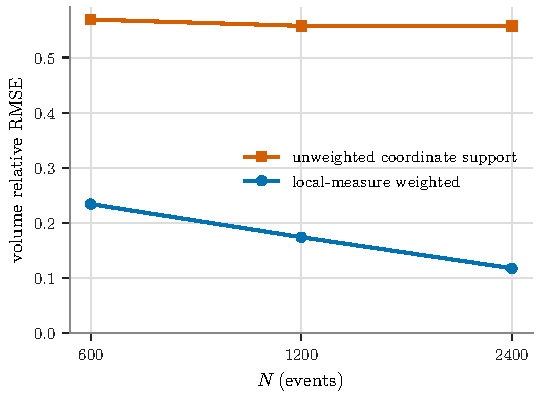
\includegraphics[width=0.95\textwidth]{figures/fig3_measure.pdf}
\caption{R5: what the local measure buys. For the position-dependent
profile, the unweighted estimate's relative error stalls at a floor that no
global recalibration removes, while the weighted estimate falls with $N$
onto the flat-profile sampling floor (a); panel (b) shows the same
comparison in absolute volume RMSE on logarithmic axes, where the two carry
visibly different slopes. The constant-profile arm is not plotted---it is a
normalization identity, R1's ingredient (\sref{sec:r5}). Order alone fixes
no absolute scale, and no scale alone fixes a profile.}
\label{fig:measure}
\end{figure}

\subsection{Horizon analogue --- Rindler reconstruction-inaccessibility}\label{sec:rindler}

For an accelerated (Rindler) observer in flat spacetime, two-way radar
reconstruction is confined to the Rindler wedge, and nothing leaks out of it:
in every configuration the classification records zero false positives and
zero false negatives, precision $=$ recall $= 1.0$. That scoring is against
the events finite clock coverage makes accessible, not against the ideal
wedge; measured against the ideal wedge the same reconstruction is incomplete,
recovering a fraction 0.74 to 0.84 of it, because part of the wedge lies
beyond the observer's tick range. The wedge itself covers about a quarter of
events (accessible fraction ${\sim}0.25$), and the in-wedge radar-time RMSE
falls with tick resolution (e.g.\ $0.0098 \to 0.0023$)
(\expid{exp16};
\artifact{outputs/\allowbreak{}data/\allowbreak{}rindler\_\allowbreak{}horizon\_\allowbreak{}reconstruction\_\allowbreak{}summary.csv}).
Comparing observers directly, all events are accessible to the inertial
observer while only ${\sim}0.25$ (ideal wedge) / ${\sim}0.21$ (finite clock
coverage) are accessible to the Rindler observer, and no event is
Rindler-accessible but inertial-inaccessible---a strict subset (\expid{exp17};
\artifact{outputs/\allowbreak{}data/\allowbreak{}inertial\_\allowbreak{}vs\_\allowbreak{}rindler\_\allowbreak{}accessibility.csv}). This is a
controlled flat-spacetime horizon analogue, not a black-hole simulation.
